\documentclass[a4paper,
fontsize=11pt,
%headings=small,
oneside,
numbers=noperiodatend,
parskip=half-,
bibliography=totoc,
final
]{scrartcl}

\usepackage[babel]{csquotes}
\usepackage{synttree}
\usepackage{graphicx}
\setkeys{Gin}{width=.4\textwidth} %default pics size

\graphicspath{{./plots/}}
\usepackage[ngerman]{babel}
\usepackage[T1]{fontenc}
%\usepackage{amsmath}
\usepackage[utf8x]{inputenc}
\usepackage [hyphens]{url}
\usepackage{booktabs} 
\usepackage[left=2.4cm,right=2.4cm,top=2.3cm,bottom=2cm,includeheadfoot]{geometry}
\usepackage[labelformat=empty]{caption} % option 'labelformat=empty]' to surpress adding "Abbildung 1:" or "Figure 1" before each caption / use parameter '\captionsetup{labelformat=empty}' instead to change this for just one caption
\usepackage{eurosym}
\usepackage{multirow}
\usepackage[ngerman]{varioref}
\setcapindent{1em}
\renewcommand{\labelitemi}{--}
\usepackage{paralist}
\usepackage{pdfpages}
\usepackage{lscape}
\usepackage{float}
\usepackage{acronym}
\usepackage{eurosym}
\usepackage{longtable,lscape}
\usepackage{mathpazo}
\usepackage[normalem]{ulem} %emphasize weiterhin kursiv
\usepackage[flushmargin,ragged]{footmisc} % left align footnote
\usepackage{ccicons} 
\setcapindent{0pt} % no indentation in captions
\usepackage{xurl} % Breaks URLs

%%%% fancy LIBREAS URL color 
\usepackage{xcolor}
\definecolor{libreas}{RGB}{112,0,0}

\usepackage{listings}

\urlstyle{same}  % don't use monospace font for urls

\usepackage[fleqn]{amsmath}

%adjust fontsize for part

\usepackage{sectsty}
\partfont{\large}

%Das BibTeX-Zeichen mit \BibTeX setzen:
\def\symbol#1{\char #1\relax}
\def\bsl{{\tt\symbol{'134}}}
\def\BibTeX{{\rm B\kern-.05em{\sc i\kern-.025em b}\kern-.08em
    T\kern-.1667em\lower.7ex\hbox{E}\kern-.125emX}}

\usepackage{fancyhdr}
\fancyhf{}
\pagestyle{fancyplain}
\fancyhead[R]{\thepage}

% make sure bookmarks are created eventough sections are not numbered!
% uncommend if sections are numbered (bookmarks created by default)
\makeatletter
\renewcommand\@seccntformat[1]{}
\makeatother

% typo setup
\clubpenalty = 10000
\widowpenalty = 10000
\displaywidowpenalty = 10000

\usepackage{hyperxmp}
\usepackage[colorlinks, linkcolor=black,citecolor=black, urlcolor=libreas,
breaklinks= true,bookmarks=true,bookmarksopen=true]{hyperref}
\usepackage{breakurl}

%meta
%meta

\fancyhead[L]{Ioanna Danai Katsougiannopoulou, Nadja Hartwich, Ha Thao Suong Vu\\ %author
LIBREAS. Library Ideas, 47 (2025). % journal, issue, volume.
\href{https://doi.org/10.18452/x}{\color{black}https://doi.org/10.18452/x}
{}} % doi 
\fancyhead[R]{\thepage} %page number
\fancyfoot[L] {\ccLogo \ccAttribution\ \href{https://creativecommons.org/licenses/by/4.0/}{\color{black}Creative Commons BY 4.0}}  %licence
\fancyfoot[R] {ISSN: 1860-7950}

\title{\LARGE{Digital Footprint – Choose your own adventure}}% title
\subtitle{Konzeption eines Spiels zum Thema Data Tracking in der Wissenschaft, speziell von wissenschaftlichen Verlagen für naturwissenschaftliche Early Career Researcher an Institutionen}
\author{Ioanna Danai Katsougiannopoulou, Nadja Hartwich, Ha Thao Suong Vu} % author

\setcounter{page}{1}

\hypersetup{%
      pdftitle={Digital Footprint – Choose your own adventure. Konzeption eines Spiels zum Thema Data Tracking in der Wissenschaft, speziell von wissenschaftlichen Verlagen für naturwissenschaftliche Early Career Researcher an Institutionen},
      pdfauthor={Ioanna Danai Katsougiannopoulou, Nadja Hartwich, Ha Thao Suong Vu},
      pdfsubject={LIBREAS. Library Ideas, 47 (2025)},
      pdfkeywords={Data Tracking, Workshop, Spielkonzept, Projektbericht},
      pdflicenseurl={https://creativecommons.org/licenses/by/4.0/},
      pdfcopyright={CC BY 4.0 International},
      pdfcontacturl={http://libreas.eu},
      pdfurl={},
      pdfdoi={},
      pdflang={de},
      pdfmetalang={de}
     }



\date{}
\begin{document}

\maketitle
\thispagestyle{fancyplain} 

%abstracts
\begin{abstract}
\noindent
\textbf{Zusammenfassung}: Publizieren ist für Wissenschaftler*innen
essentiell. Dabei ist es heutzutage kaum möglich, an digitalen Angeboten
vorbeizukommen. Nur wenigen Forschenden ist dabei bewusst, dass auch bei
digitalen Verlagsangeboten persönliche Daten getrackt und missbraucht
werden können.

Ein Auftrag von Bibliotheken ist es, Forschende zu unterstützen und
Informationskompetenz zu stärken. Deshalb fällt das Stärken von
Bewusstsein für Data Tracking durch wissenschaftliche Verlage in ihr
Aufgabengebiet. Dies kann unter anderem durch Workshops passieren.
Unsere Frage hierbei ist, wie Wissenschaftler*innen, speziell Early
Career Researchers in den Naturwissenschaften, Datentracking durch
wissenschaftliche Verlage, die negativen Auswirkungen und
Abwehrmöglichkeiten gegen Datentracking vermittelt werden können. In
unserem Workshop-Konzept haben wir zusätzlich zu Kurzvorträgen ein Spiel
als eine simulationsbasierte Aufgabe mit Rollenspiel-ähnlichen Merkmalen
entwickelt, das auf einem Entdecken-lassenden-Ansatz basiert. Mithilfe
dessen wird ein realitätsnaher Publikationsprozess durchgespielt. Hier
werden, abhängig von den getroffenen Entscheidungen, personenbezogene
Daten getrackt.

Dieses Konzept wurde in einem Pre-ISI-Workshop (ISI = Internationales
Symposium für Informationswissenschaft) am 17. März 2025 vorgestellt und
durchgeführt; das prototypische Kartenspiel wurde getestet und Feedback
eingeholt. Dieses Kartenspiel wird für die Weiterverwendung (und
Weiterentwicklung) als Open Educational Resource freigegeben. Mögliche
Anpassungen sind beispielsweise, den Workshop auch auf Studierende
auszurichten und ihnen so den Publikationsprozess oder den
Schreibprozess von wissenschaftlichen Arbeiten spielerisch darzustellen.

\begin{center}\rule{0.5\linewidth}{0.5pt}\end{center}

\noindent
\textbf{Abstract}: No researcher can avoid publishing. Nowadays, it is
almost impossible to avoid digital publication services. Not many people
are aware that personal data can be tracked by academic publishers
without the knowledge of the user and, in the worst case, misused. One
of the missions of libraries is to support researchers and foster
information literacy. Awareness of data tracking in scholarly publishing
houses falls within this scope. This can, for instance, be communicated
through workshops. The question here is, how scientists, especially
early career researchers in natural sciences, can be educated about data
tracking by scholarly publishing houses, along with its negative effects
and ways to defend against data tracking.

In our workshop concept, in addition to short presentations, we have
developed a game as a simulation-based task with role-playing game-like
features based on a discovery approach. This is used to play through a
reality-based publication process. Depending on the decisions made,
personal data will be tracked.

This concept was presented and implemented in the pre-ISI workshop (ISI
= International Symposium on Information Science) on March 17th, 2025,
where the prototype card game was tested, and feedback was obtained. The
card game will be released for further use (and adaptations) as an open
educational resource. Possible adaptations include targeting the
workshop towards students and thus presenting the publication process or
the writing process of academic papers to them in a playful way.
\end{abstract}

%body
\section{1 Einleitung und
Hintergrund}\label{einleitung-und-hintergrund}

Publizieren ist für Wissenschaftler*innen essentiell. Ohne Publikationen
ist es schwierig, Reputation aufzubauen, die wiederum ein Grundbaustein
für die weitere Anstellung an Institutionen ist.

Nur wenigen Wissenschaftler*innen ist bewusst, dass bei der für das
Publizieren notwendigen Nutzung von digitalen Verlagsangeboten
persönliche Daten getrackt werden. Persönliche Daten sind allerdings
unter dem Recht auf informationelle Selbstbestimmung geschützt (in
Deutschland GG, 2022, §~2, Abs.~1 in Verbindung mit GG, 2022, §~1
Abs.~1, in anderen europäischen Ländern in Gesetzen mit ähnlichem Ziel).
Dabei handelt es sich um ein Recht, das im Datenschutz verankert ist.

Dennoch legen kommerzielle Firmen, wozu auch einige wissenschaftliche
Verlage gehören, dieses Recht immer wieder möglichst weit aus. Die
getrackten persönlichen Daten können im schlimmsten Fall missbraucht
werden.\footnote{DFG-Ausschuss für Wissenschaftliche Bibliotheken und
  Informationssysteme, \enquote{Datentracking in der Wissenschaft:
  Aggregation und Verwendung bzw. Verkauf von Nutzungsdaten durch
  Wissenschaftsverlage. Ein Informationspapier des Ausschusses für
  Wissenschaftliche Bibliotheken und Informationssysteme der Deutschen
  Forschungsgemeinschaft}, 28. Juli 2021,
  \url{https://doi.org/10.5281/zenodo.5900759}, S.~5.} Dies kann zum
Beispiel zu Deportationen von immigrierten Wissenschaftler*innen
führen.\footnote{Sam Biddle, \enquote{LexisNexis to Provide Giant
  Database of Personal Information to ICE}, The Intercept, 2. April
  2021,
  \url{https://theintercept.com/2021/04/02/ice-database-surveillance-lexisnexis/}.}

Auf wissenschaftlichen Verlagsseiten werden u.a. Profile, Nutzungsdaten,
Seitenbesuche etc. gespeichert.\footnote{DFG-Ausschuss Für
  Wissenschaftliche Bibliotheken Und Informationssysteme,
  \enquote{Datentracking in der Wissenschaft}. S.~3~f.} Diese können an
Data Broker gelangen, welche diese wiederum an bspw. in den USA an eine
Deportationsbehörde verkauft werden könnten, wodurch eine Gefahr für
Wissenschaftler*innen entstehen kann.\footnote{Biddle,
  \enquote{LexisNexis to Provide Giant Database of Personal Information
  to ICE}.} Ein weiteres Beispiel kommt aus der Rechtsberatung, das im
folgenden Beispiel\footnote{Lamdan, \enquote{When Westlaw Fuels ICE
  Surveillance: Legal Ethics in the Era of Big Data Policing}.}
nachgelesen werden kann.

Ein Auftrag von Bibliotheken ist es, Forschende zu unterstützen und
Informationskompetenz zu stärken.\footnote{dbv,
  \enquote{Wissenschaftliche Bibliotheken 2025 - Strategiepapier zur
  Gestaltung von Zukunftsaufgaben im wissenschaftlichen
  Bibliothekswesen} (Deutscher Bibliotheksverband, 7. Februar 2022),
  \url{https://www.bibliotheksverband.de/sites/default/files/2022-02/Strategiepapier_Wissenschaftliche\%20Bibliotheken\%202025\%20-\%20FINAL.pdf},
  S.~9.} Dabei fällt ein Bewusstsein für Data Tracking in
wissenschaftlichen Verlagen unter ihr Aufgabengebiet. Diese Vermittlung
kann u.a. durch Workshops passieren. Aus diesem Grund haben wir uns
entschieden, einen Workshop für Early Career Researchers zu gestalten,
der gerade für diese Thematik sensibilisiert. Unsere Frage hierbei ist,
wie Wissenschaftler*innen in den Naturwissenschaften Data Tracking in
wissenschaftlichen Verlagen, sowie deren negative Auswirkungen und
Abwehrmöglichkeiten gegen Data Tracking vermittelt werden kann.

Im Rahmen des an der Fachhochschule Potsdam durchgeführten Kurses
\enquote{B 12: Informationsdidaktik und Informationskompetenz} unter der
Leitung von Prof.~Dr.~Ulrike Wuttke und dem Praxispartner Dr.~Timo
Steyer wurde zum Thema Data Tracking in der Wissenschaft ein
Workshop-Konzept entwickelt, das auf naturwissenschaftliche Early Career
Researcher an Institutionen ausgerichtet ist. Ein Teil dieses Konzepts
ist ein Kartenspiel mit Rollenspiel-ähnlichen Merkmalen.

Wir, die Autor*innen, haben uns aufgrund bereits erworbener Erfahrungen
im Schulungsbereich sowie in der Arbeit mit naturwissenschaftlichen
Instituten für diese Methode entschieden, um ein möglichst praxisnahes
Konzept zu entwickeln.

Als Ziel wurde eine erhöhte Sensibilisierung der Teilnehmer*innen für
das Thema Data Tracking wissenschaftlicher Verlage festgesetzt. Zudem
wurde durch die Wahl eines spielerischen Ansatzes eine erhöhte
Wissensfestigung und Beteiligung am Workshop angestrebt.\footnote{Tobias
  Seidl, \enquote{Didaktische Grundlagen}, in \emph{Handbuch
  Bibliothekspädagogik} (De Gruyter Saur, 2024), 119--28,
  \url{https://doi.org/10.1515/9783111032030-011}.}

Dieses Konzept wurde in einem Pre-ISI-Workshop (ISI = Internationales
Symposium für Informationswissenschaft) am 17. März 2025 vorgestellt und
durchgeführt. Das prototypische Kartenspiel wurde getestet und Feedback
eingeholt.

\section{2 Konzept des Spiels}\label{konzept-des-spiels}

Der Workshop richtet sich explizit an die Zielgruppe Early Career
Researchers, die in naturwissenschaftlichen Institutionen tätig sind.

Zudem beschränken wir uns auf das Forschungsfeld der
Naturwissenschaften. Wir haben uns für diese Gruppe entschieden, da wir
sowohl im akademischen, beruflichen als auch im persönlichen Umfeld oft
mit dieser Gruppe zu tun haben.

Um die Relevanz des Themas Data Tracking in wissenschaftlichen Verlagen
auch der definierten Zielgruppe näher zu bringen, wurde zuerst ein
Lernziel gebildet. Dieses lautet:

\begin{displayquote}
\emph{Die Lernenden sind sich des Data Tracking durch wissenschaftliche
Verlage und dessen negativen Auswirkungen sowie der Abwehrmöglichkeiten
gegen Data Tracking bewusst.}
\end{displayquote}

\subsection{2.1 Idee}\label{idee}

Das Konzept des Kartenspiels orientiert sich an dem
\enquote{Du-entscheidest-selbst-Prinzip} beziehungsweise \enquote{Choose
Your Own Adventure}-Prinzip,\footnote{Eli Cook, \enquote{Rearing
  Children of the Market in the}You'' Decade: Choose Your Own Adventure
  Books and the Ascent of Free Choice in 1980s America'', \emph{Journal
  of American Studies} 55, Nr. 2 (Mai 2021): 418--45,
  \url{https://doi.org/10.1017/S0021875819001476}.} das unter anderem in
der Buchreihe \enquote{1000 Gefahren} genutzt wird. In diesen werden
kurze Textabschnitte gelesen, an dessen Ende Entscheidungen gefällt
werden können. Abhängig von der Entscheidung ändert sich der Verlauf der
Geschichte.

Auch in unserem Kartenspiel entscheiden die Spielenden, in welche
Richtung die \enquote{Geschichte} gehen soll. Bei der
\enquote{Geschichte} des Kartenspiels begleiten die Spielenden eine*n
Wissenschaftler*in, der*die eine Doktorarbeit schreiben möchte. Es fängt
mit der Auswahl des Forschungsthemas an und endet mit einer fertig
geschriebenen Arbeit.

Teilnehmende werden in Gruppen von zwei bis vier Personen eingeteilt.
Einerseits soll dadurch der Austausch zwischen den Teilnehmenden
unterstützt und ein Ausgleich von unterschiedlichen Wissensständen
ermöglicht werden. Dadurch, dass die Entscheidungen in einer Gruppe
getroffen werden, kann die Scheu eliminiert werden, die
\enquote{falschen} Entscheidungen zu treffen und somit
\enquote{schlechtere Ergebnisse} bei der Gruppendiskussion vorstellen zu
müssen.

Im Laufe des Spiels werden an verschiedenen Punkten Daten getrackt, die
in einem Arbeitsblatt vermerkt werden, und somit den Spielenden
verdeutlichen, welche Daten bei einem digitalen Rechercheprozess
möglicherweise preisgegeben werden.

Im Anschluss an das Spiel findet ein Austausch über die Spielergebnisse
statt, bei dem das neu erworbene Wissen und die gewonnenen Erkenntnisse
aus dem Spiel diskutiert werden.

Das Spiel, eine simulationsbasierte Aufgabe\footnote{Ulrike Hanke,
  Martina Straub, und Wilfried Sühl-Strohmenger, \enquote{6 Lehrmethoden
  für die Realisierung von Lehrszenarien an der Teaching Library}, in
  \emph{Informationskompetenz professionell fördern} (DE GRUYTER SAUR,
  2012), 26--54, \url{https://doi.org/10.1515/9783110274387.26}.} mit
Rollenspiel\footnote{Hanke, Straub, und Sühl-Strohmenger.}-ähnlichen
Merkmalen, basiert auf einem
\enquote{entdecken-lassenden-Ansatz}\footnote{Ulrike Hanke und Wilfried
  Sühl-Strohmenger, \enquote{9. Planen und Konzipieren von
  Bildungsangeboten}, in \emph{9. Planen und Konzipieren von
  Bildungsangeboten} (De Gruyter Saur, 2015), 166--82,
  \url{https://doi.org/10.1515/9783110352559-011}.}, der es den
Teilnehmenden ermöglicht, eigenständig in Gruppen\footnote{Markus
  Brauer, \enquote{Erfolgreiche Lehrmethoden im Seminar}, in \emph{An
  der Hochschule lehren} (Springer, Berlin, Heidelberg, 2014), 69--86,
  \url{https://doi.org/10.1007/978-3-642-42006-1_6}.} mit den von den
Teamer*innen bereitgestellten Materialien zu arbeiten und so die
Anwendung von Data Tracking im wissenschaftlichen Kontext zu entdecken.
Dieses antizipatorische Lernen\footnote{\enquote{Volkshochschule
  Saale-Orla-Kreis: Qualität}, zugegriffen 8. August 2024,
  \url{https://www.vhs-sok.de/ihre-vhs/qualitaet}.} ermöglicht es den
Teilnehmenden, ihr Vorwissen zu aktivieren. Da das Spiel die
Teilnehmenden in einer authentischen Situation agieren lässt, eine
aktive Beteiligung anregt und keinen festen Lösungsweg vorsieht, wodurch
es am Ende weder Gewinner noch Verlierer gibt, ist dieser Ansatz
sinnvoll.

\subsection{2.2 Prozess}\label{prozess}

Bei der Konzipierung des Spiels gab es einige Ideen, die nicht alle
verwendet wurden.

Eine davon war es, den Spielenden verschiedene Personas beziehungsweise
\enquote{Spielcharaktere} zu geben. Dies würde aber das Spiel
komplizierter gestalten und eventuell die Spielenden dazu verleiten,
nicht \enquote{sich selbst} zu spielen, sondern den Charakter und somit
andere Entscheidungen zu treffen. Deswegen wurde dieses Konzept nicht
weiter ausgearbeitet.

Eine weitere Idee war es, auf der Rückseite der Karten weiterführende
Quellen dazu anzugeben, wieso bei dieser Entscheidung diese persönlichen
Daten getrackt werden. Jedoch würden diese Quellenangaben den Spielfluss
unterbrechen und die Karte zu sehr mit Informationen überladen.

Die Sprache des Spiels war auch ein Diskussionspunkt. Die Entscheidung
lag zwischen Deutsch und Englisch. Schlussendlich hatten wir uns für
Englisch entschieden, weil die Naturwissenschaften ein internationales
Feld sind, in dem Englisch die Hauptkommunikationssprache darstellt.

Das endgültige Konzept des Spiels beinhaltet eine Spielanleitung,
(leere) Worksheets, in denen die getrackten Daten vermerkt werden
können, ein ausgefülltes Worksheet für die Teamer*innen zur Kontrolle,
ein beispielhafter Aufbau des Spiels, und die Karten, die jeweils aus
einem Stapel von Frage- und Antwortkarten bestehen.

Unser erstes Konzept der Karten sah wie folgt aus.

\begin{figure}[H]
\centering
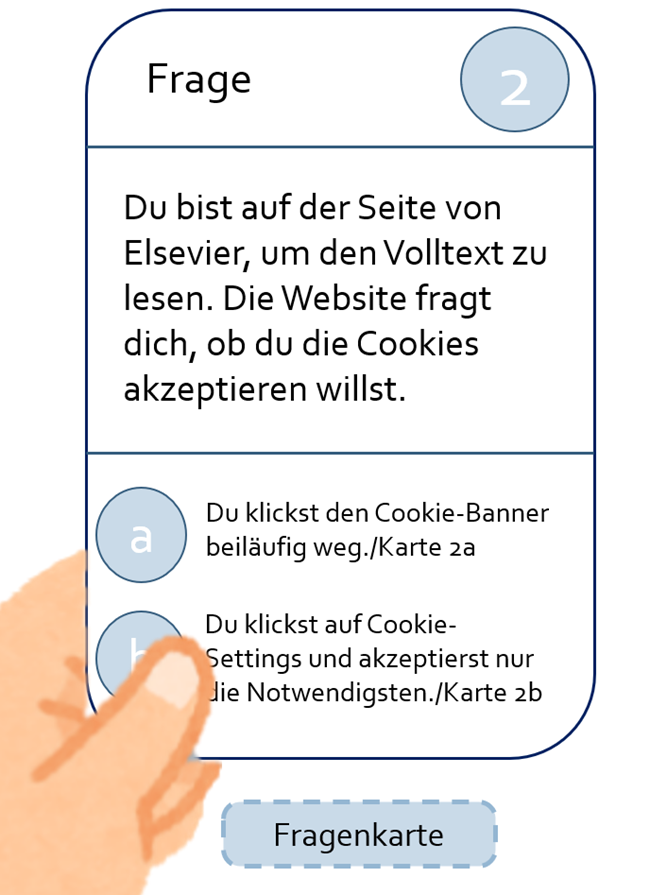
\includegraphics[width=.3\textwidth]{img/Abb1-Fragekarte.png}
\caption{Abbildung 1: Konzept Fragenkarte, Quelle: Eigene Darstellung}
\end{figure}

Abbildung 1 zeigt die Fragekarte. Sowohl die Farbe als auch der Text
oben links verdeutlicht, dass dies die Fragekarte ist. Mittig wird die
\enquote{Story} gezeigt, und unter dieser werden je zwei
Antwortmöglichkeiten und dessen Nummerierung abgebildet.

\begin{figure}[H]
\centering
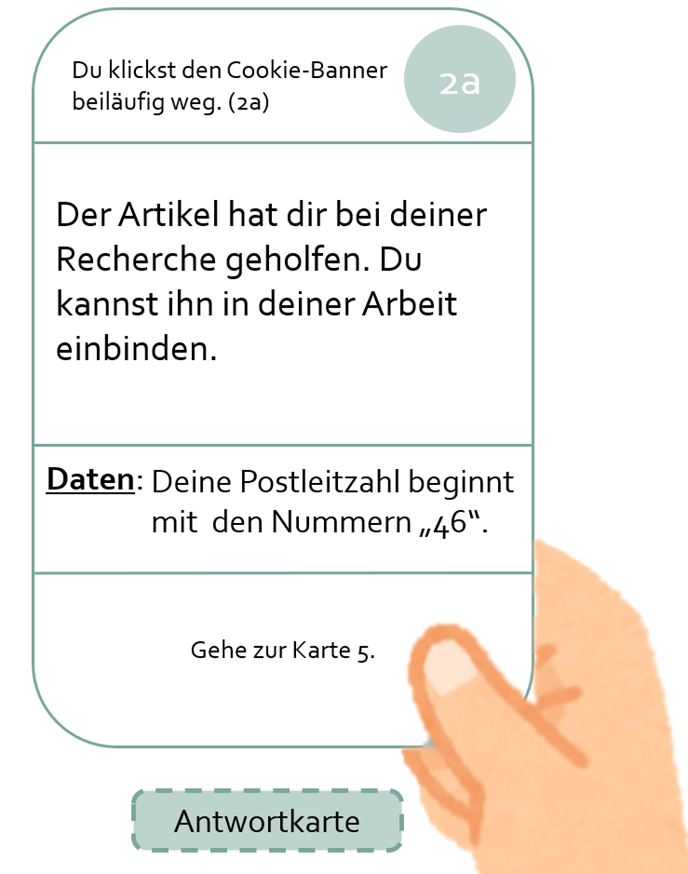
\includegraphics[width=.3\textwidth]{img/Abb2-Antwortkarte.png}
\caption{Abbildung 2: Konzept Antwortkarte, Quelle: Eigene Darstellung}
\end{figure}

In Abbildung 2 ist das erste Konzept der Antwortkarte. Bei dieser ist
oben sowohl die Kartennummer als auch die getroffene Entscheidung zu
sehen. Unter diesen ist die Konsequenz in Textform zusammen mit den
getrackten Daten dargestellt. Im unteren Abschnitt der Karte wird auf
die nächste Karte, die gezogen werden soll, hingewiesen.

Beim Endprodukt (siehe Abbildungen 3 und 4) wurden pragmatische
Entscheidungen hinsichtlich des Designs getroffen. Beispielsweise wurden
die abgerundeten Ecken, die wir ästhetischer finden, gestrichen. Der
Grund hierbei ist, dass das Kartenspiel selbst druckbar sein sollte.
Abgerundete Ecken würden hierbei ein Mehraufwand beim Schneideprozess
sein. Dazu wurden die Farben so ausgewählt, dass die Frage- und
Antwortkarten auch für farbblinde Menschen gut erkennbar beziehungsweise
wenn die Karten in Graustufen gedruckt werden, diese trotzdem
unterscheidbar sind. Auf einem A4-Blatt können acht Karten gedruckt
werden.

\begin{figure}[H]
\centering
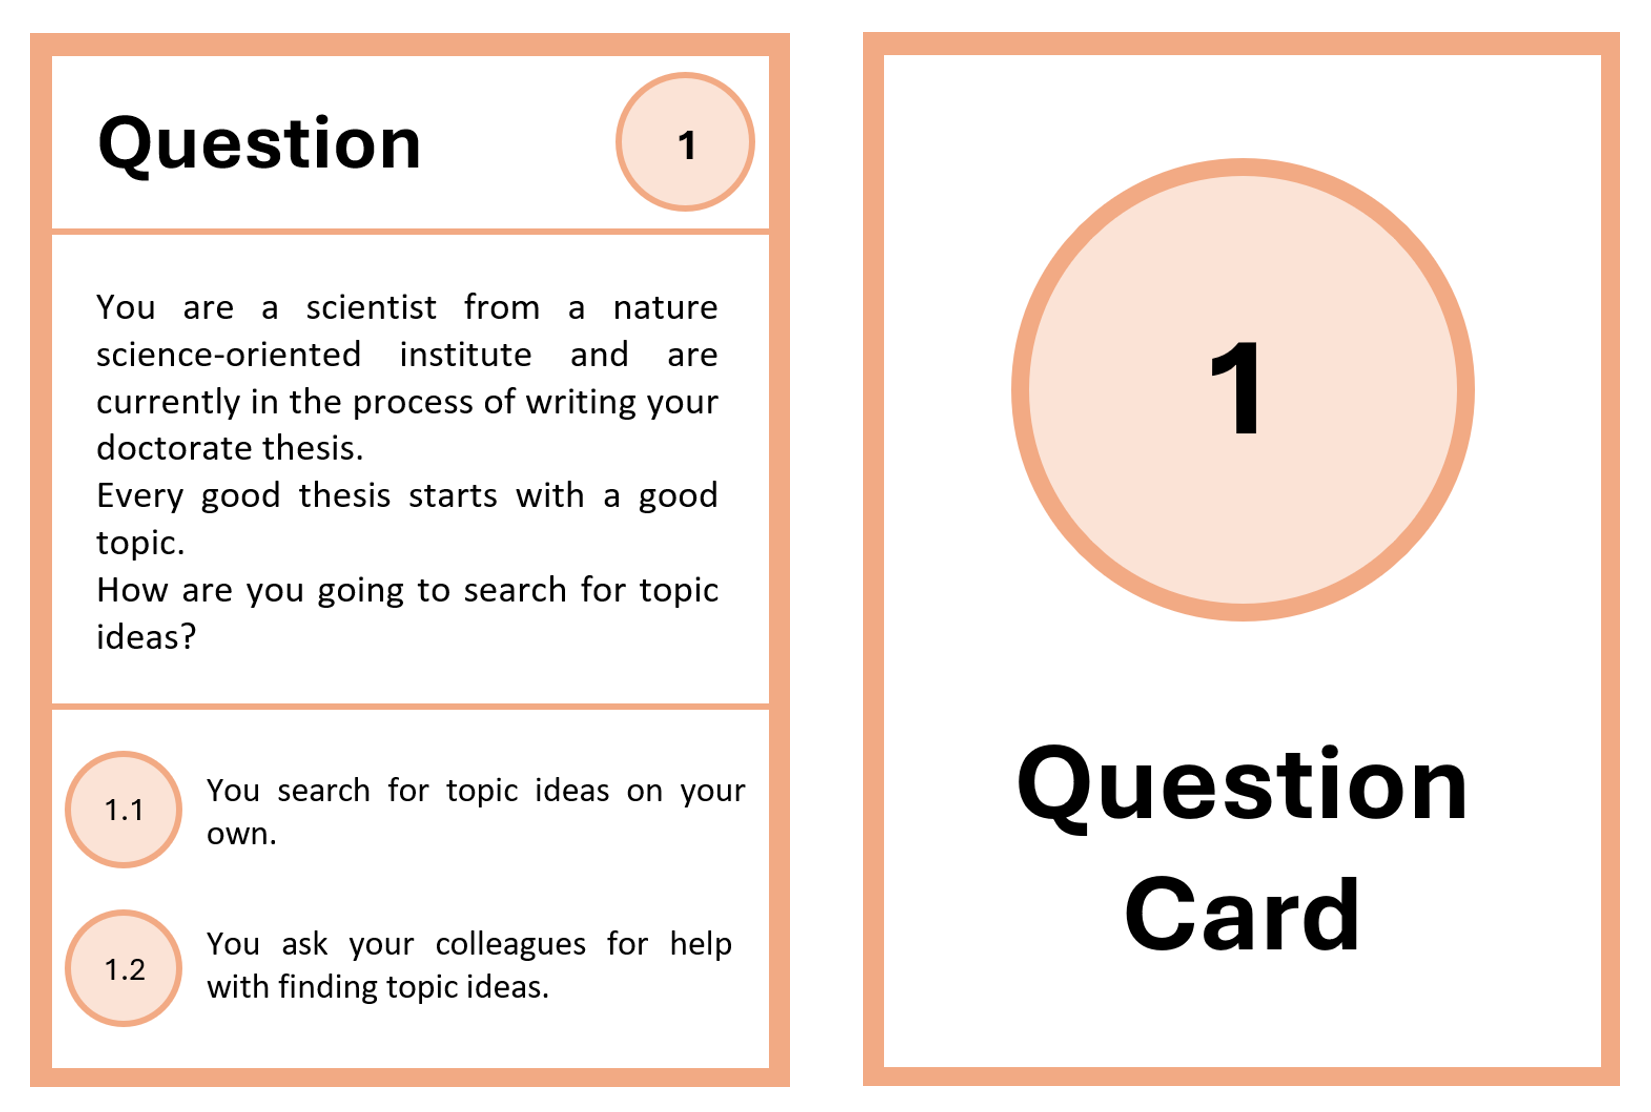
\includegraphics[width=.5\textwidth]{img/Abb3.png}
\caption{Abbildung 3: Endprodukt Fragenkarte, Quelle: Eigene
Darstellung}
\end{figure}

\begin{figure}[H]
\centering
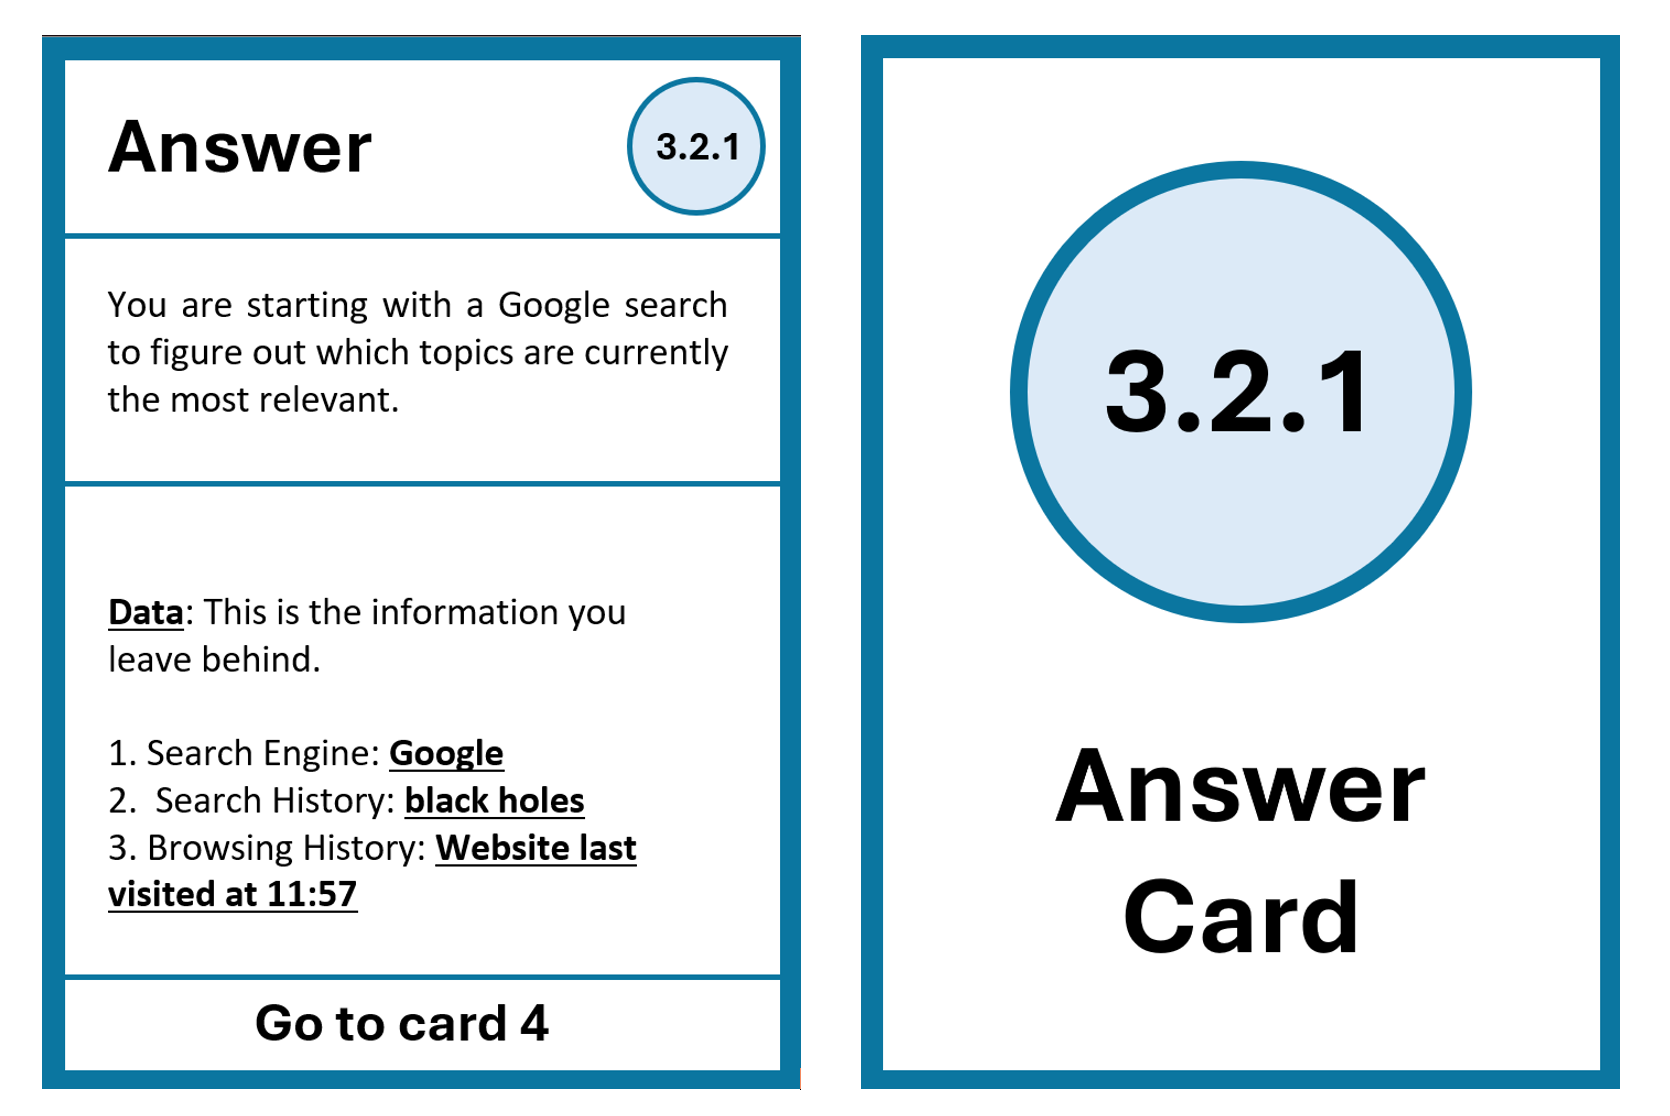
\includegraphics[width=.5\textwidth]{img/Abb4.png}
\caption{Abbildung 4: Endprodukt Antwortkarte, Quelle: Eigene
Darstellung}
\end{figure}

Die Storyline, der Text der Karten, zusammen mit den getrackten Daten
und die Entscheidungspfade wurden in einem Baumdiagramm erfasst.

\begin{figure}[H]
\centering
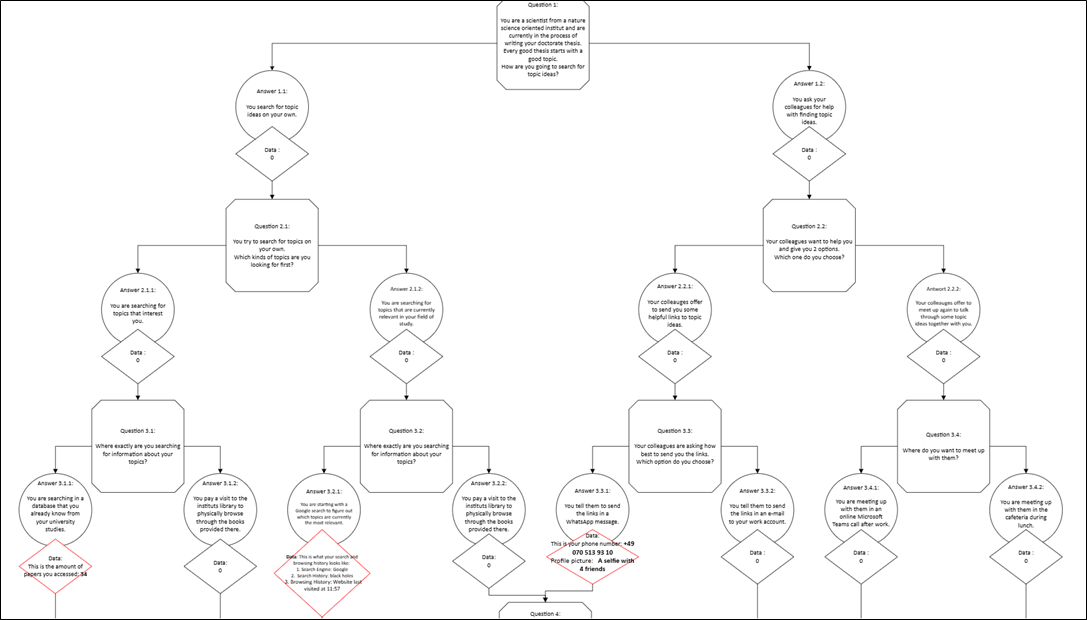
\includegraphics[width=1\textwidth]{img/Abb5-Baumdiagram.png}
\caption{Abbildung 5: Ausschnitt des Baumdiagramm (zur Veranschaulichung
der Komplexität), Quelle: Eigene Darstellung}
\end{figure}

Vor dem Spiel wird dieses aufgebaut.

\begin{figure}[H]
\centering
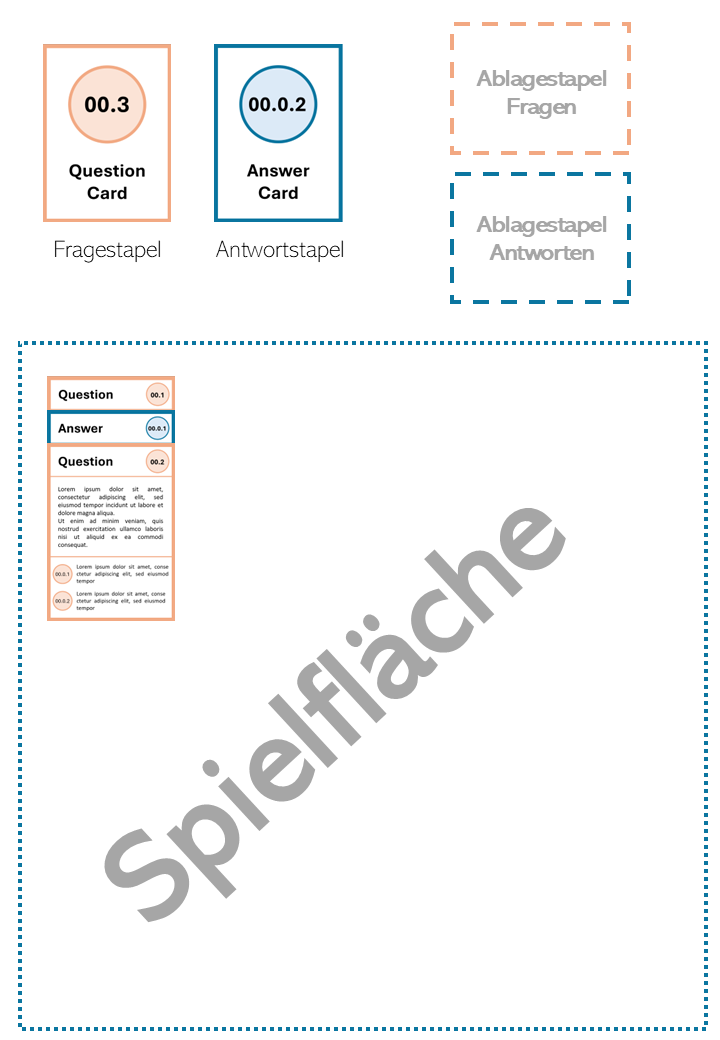
\includegraphics[width=.5\textwidth]{img/Abb6-Spielablauf.png}
\caption{Abbildung 6: Darstellung des Spielablaufs, Quelle: Eigene
Darstellung}
\end{figure}

Links oben wird je ein Stapel von Frage- und Antwortkarten gebildet. Bei
diesen sollte die Rückseite, auf der die Nummer groß zu sehen ist,
sichtbar sein. Rechts oben, neben den Frage- und Antwortkarten, wird
sich im Laufe des Spiels je ein Ablagestapel bilden. Unter diesen vier
Stapeln befindet sich die Spielfläche, auf welcher die Karten, der
Reihenfolge nach, gelegt werden.

\subsection{2.3 Erste Durchführung des
Spiels}\label{erste-durchfuxfchrung-des-spiels}

Im Zuge einer Movetia-Partnerschaft von der FH Potsdam mit der FH
Graubünden wurde am 17. März 2025 ein Pre-ISI-Workshop (ISI =
Internationales Symposium für Informationswissenschaft) veranstaltet, in
dem das Kartenspiel getestet wurde. Näheres hierzu kann in dieser
LIBREAS-Ausgabe bei Wuttke nachgelesen werden
(\url{https://libreas.eu/ausgabe47/wuttke}).

Hierbei haben sich zwei Gruppen gebildet. In einer Gruppe waren vier
Studierende aus der FH Potsdam und in der zweiten Gruppe waren insgesamt
sechs Personen plus ein Online-Teilnehmender, die Lehrende oder andere
Personen aus der informationswissenschaftlichen Praxis waren. Somit
waren die Teilnehmenden nicht die Zielgruppe, sodass die Ergebnisse
nicht 1-zu-1 übertragbar sind. Jedoch konnte so eine weitere Sichtweise
auf das Spiel ermittelt werden.

Um eine möglichst realitätsnahe Erfahrung zu schaffen, wurden die Regeln
im Vorhinein nicht explizit von uns erklärt. Stattdessen haben die
Teilnehmer*innen eigenständig die Spielanleitung gelesen, um mögliche
Verständnisschwierigkeiten zu ermitteln. Bei Fragen und Unklarheiten
standen wir zur Verfügung.

Die Stimmung während des Spiels war positiv. Einige Stellen wurden
humorvoll kommentiert. Beispiele für Reaktionen sind (sinngemäß):
\enquote{Wir nehmen LaTeX, wir sind Profis.} oder \enquote{Online. Ich
geh doch nicht extra in eine Library.} Ein weiterer Ausruf war:
\enquote{Ich geh zum Koordination-Office, vielleicht gibt es da Geld.}
Die Interaktion zwischen den Teilnehmenden führte zu Diskussionen, die
unter anderem mit Abstimmungen und Kommentaren wie \enquote{Verräter}
auf eine heitere Atmosphäre hindeuteten. Manche Entscheidungen haben
emotionale Reaktionen ausgelöst. So wurde bei der Frage \enquote{You go
to the website and the cookie banner appears. What do you do?} die
trockene Antwort \enquote{Scream.} gegeben.

Konzeptuell wurde das Spiel auf 45 min angesetzt. Die eigentliche
Spielzeit war zwischen 47 Minuten bis zu einer Stunde, jedoch war die
zweite Gruppe auch größer und somit diskussionsfreudiger als im Konzept
vorgesehen war.

Während des Spiels gab es kleinere Verständnisfragen, die mit einer
Überarbeitung des Textes eliminiert werden können.

Beim Feedback wurde zurückgemeldet, dass das Spiel Spaß gemacht und
insgesamt einen positiven Eindruck hinterlassen hatte. Ein
Diskussionspunkt war, dass im Spiel konkrete Software, Webseiten und
ähnliches genannt wurde. Dies ist zwar einerseits realitätsnah,
andererseits sind diese den Teilnehmenden eventuell unbekannt. Die
Lösung hierfür war, den Namen kurze Erläuterungen hinzuzufügen.

Auch die kontinuierliche Aktualisierung des Spiels wurde thematisiert,
da sich vor allem digitale Tools und Produkte mit der Zeit ändern. Dies
sollte bei der Aktualisierung des Gesamtkonzepts des Workshops beachtet
werden, die bestenfalls alle zwei Jahre stattfinden sollte.

Eine Frage unsererseits an die Teilnehmenden war, ob und in welcher Form
wir eine Quellenangabe zu den getrackten Daten erstellen sollten. Der
Vorschlag, dies in Form einer Zusatzkarte beziehungsweise eines
Handbuchs anzufertigen, wurde positiv angenommen. Ein genannter Grund
war, dass der Spielfluss somit nicht durch eine Überladung von
Informationen unterbrochen wird. Dazu werden die Teilnehmenden angeregt,
selbst weiter zu recherchieren.

\section{3 Learnings}\label{learnings}

Eine Herausforderung bei der Konzipierung war es, die Kontinuität der
Informationen und Daten sicherzustellen, sodass zum Beispiel nicht
mitten in der \enquote{Geschichte} der Browser wechselt. Zudem sollte
auf die Sprache geachtet werden. Begriffe wie \enquote{googeln} werden
in einer Generation beispielsweise als Synonym für
\enquote{recherchieren} genutzt, während eine andere Generation dies
eher mit einer Sucheingabe in Google verbindet.

Der Aufwand, das Spiel zu erarbeiten, war hoch. Einerseits mussten die
getrackten Daten, welche von Verlagen getrackt werden (können),
recherchiert und dies mit fundierten Quellen belegt werden. Andererseits
musste eine Storyline mit einem roten Faden entwickelt werden. Diese
Informationen mussten sinnvoll kombiniert werden, um eine realitätsnahe
Spielerfahrung zu ermöglichen. Gleichzeitig musste beachtet werden, dass
die Inhalte des Spiels verständlich aufbereitet werden und bei den
Spielenden ein Lerneffekt entsteht, während das Spiel unterhaltsam
bleibt.

Wir hatten uns auch zum Ziel gesetzt, dass wir das Spiel als eine
Vorlage bereitstellen und diese von Institutionen angepasst und
weiterverwendet werden können. Dabei wurden unter anderem Vorlagen für
die Karten erstellt. Hierbei mussten die Vorder- und Hinterseiten so
positioniert werden, dass sie übereinstimmen. Je nach Drucker kann dies
unterschiedlich schwer sein. Es ist ratsam, die Karten professionell
drucken zu lassen. Zudem bietet sich stabiles Papier oder eine
Laminierung an, um die Karten wiederholt nutzen zu können.

Die analoge Form des Spiels wurde positiv aufgenommen und bestätigt
somit die Wahl dieses Formats. In der Diskussion wurde angerissen, ob
eine digitale Version entwickelt werden sollte. Da aber unsere
Zielgruppe viel digital arbeitet, kann das physische Spielen eine schöne
Abwechslung zum Arbeitsalltag darstellen.

\section{4 Ausblick}\label{ausblick}

Während der Diskussion kamen Vorschläge für die Professionalisierung
auf. Einer dieser war die Verbindung von Storyline-Diagramm mit den
Karten, sodass Änderungen im Diagramm gleich im Kartentext übernommen
werden. Ein weiterer Vorschlag war es, das Kartenspiel durch einen
Spieleverlag professionell verlegen zu lassen.

Inhaltlich kann das Kartenspiel auch eine Erweiterungsstufe für
Fortgeschrittene bekommen. Ein andere Nachnutzungsmöglichkeit wäre,
weitere Storylines zu entwickeln. Ein Beispiel ist, das Kartenspiel zu
nutzen, um Studienanfänger*innen den wissenschaftlichen Schreibprozess
bei Hausarbeiten näherzubringen oder einer jüngeren Zielgruppe einen
Einstieg in Informationskompetenz im Web zu geben.

Es ist beabsichtigt, das Konzept, sowie die dazugehörigen Materialien
als Open Educational Resources (OER) unter der offenen Lizenz CC BY NC
4.0 (\url{https://creativecommons.org/licenses/by-nc/4.0/})
bereitzustellen und auf Zenodo zu veröffentlichen.

\section{Quellen}\label{quellen}

Biddle, Sam. \enquote{LexisNexis to Provide Giant Database of Personal
Information to ICE}. The Intercept, 2. April 2021.
\url{https://theintercept.com/2021/04/02/ice-database-surveillance-lexisnexis/}.

Brauer, Markus. \enquote{Erfolgreiche Lehrmethoden im Seminar}. In
\emph{An der Hochschule lehren}, 69--86. Springer, Berlin, Heidelberg,
2014. \url{https://doi.org/10.1007/978-3-642-42006-1_6}.

Cook, Eli. \enquote{Rearing Children of the Market in the}You'' Decade:
Choose Your Own Adventure Books and the Ascent of Free Choice in 1980s
America''. \emph{Journal of American Studies} 55, Nr. 2 (Mai 2021):
418--45. \url{https://doi.org/10.1017/S0021875819001476}.

dbv. \enquote{Wissenschaftliche Bibliotheken 2025 - Strategiepapier zur
Gestaltung von Zukunftsaufgaben im wissenschaftlichen Bibliothekswesen}.
Deutscher Bibliotheksverband, 7. Februar 2022.
\url{https://www.bibliotheksverband.de/sites/default/files/2022-02/Strategiepapier_Wissenschaftliche\%20Bibliotheken\%202025\%20-\%20FINAL.pdf}.

DFG-Ausschuss für Wissenschaftliche Bibliotheken und
Informationssysteme. \enquote{Datentracking in der Wissenschaft:
Aggregation und Verwendung bzw. Verkauf von Nutzungsdaten durch
Wissenschaftsverlage. Ein Informationspapier des Ausschusses für
Wissenschaftliche Bibliotheken und Informationssysteme der Deutschen
Forschungsgemeinschaft}, 28. Juli 2021.
\url{https://doi.org/10.5281/zenodo.5900759}.

Hanke, Ulrike, Martina Straub, und Wilfried Sühl-Strohmenger. \enquote{6
Lehrmethoden für die Realisierung von Lehrszenarien an der Teaching
Library}. In \emph{Informationskompetenz professionell fördern}, 26--54.
DE GRUYTER SAUR, 2012. \url{https://doi.org/10.1515/9783110274387.26}.

Hanke, Ulrike, und Wilfried Sühl-Strohmenger. \enquote{9. Planen und
Konzipieren von Bildungsangeboten}. In \emph{9. Planen und Konzipieren
von Bildungsangeboten}, 166--82. De Gruyter Saur, 2015.
\url{https://doi.org/10.1515/9783110352559-011}.

Seidl, Tobias. \enquote{Didaktische Grundlagen}. In \emph{Handbuch
Bibliothekspädagogik}, 119--28. De Gruyter Saur, 2024.
\url{https://doi.org/10.1515/9783111032030-011}.

\enquote{Volkshochschule Saale-Orla-Kreis: Qualität}. Zugegriffen am 23.
September 2025. \url{https://www.vhs-sok.de/ihre-vhs/qualitaet}.

%autor
\begin{center}\rule{0.5\linewidth}{0.5pt}\end{center}

\textbf{Ioanna Danai Katsougiannopoulou} (she/they) studiert
Bibliothekswissenschaft an der Fachhochschule Potsdam. Zusätzlich zum
Studium ist Danai in verschiedenen Funktionen im Landesverband
AndersARTiG e.\,V. tätig. Hier ist Danai ein Teil des Projektes Bildung
unterm Regenbogen, indem Workshops für Schüler*innen ab der 8.
Klasse in ganz Brandenburg zum Thema sexuelle und geschlechtliche
Vielfalt angeboten werden. Dazu ist Danai Teil der
Campusspezialist*innen Team in der FH Potsdam, indem Workshops und
Schulveranstaltungen für Schüler*innen zum Thema Studium allgemein,
Studienalltag und Studienplatzsuche angeboten werden. In diesen wurden
bereits Erfahrungen zu didaktischen Ansätzen gesammelt, die im Beitrag
angewendet wurden.

ORCID: \url{https://orcid.org/0009-0008-8555-549X}

FH Potsdam ROR ID: \url{https://ror.org/012m9bp23}

\textbf{Nadja Hartwich} (sie/ihr) studiert Bibliothekswissenschaft an
der Fachhochschule Potsdam. Zusätzlich zum Studium arbeitet Nadja in der
Bibliothek des Helmholtz-Zentrum für Geoforschung in Potsdam. Viele
Erfahrungen durch die Arbeit an einem naturwissenschaftlichen Institut
sowie ein vorhergegangenes Physikstudium konnten somit in die Konzeption
des Spiels einfließen. Als früheres Mitglied des Projektes Bildung
unterm Regenbogen und ähnlichen Bildungsprojekten konnte Nadja ebenfalls
Erfahrungen zu didaktischen Ansätzen sammeln, die im Beitrag angewendet
wurden.

ORCID: \url{https://orcid.org/0009-0004-2212-5047}

FH Potsdam ROR ID: \url{https://ror.org/012m9bp23}

\textbf{Ha Thao Suong Vu} (keine Pronomen) studiert
Bibliothekswissenschaft an der Fachhochschule Potsdam. Zusätzlich zum
Studium ist Suong in verschiedenen Funktionen im Landesverband
AndersARTiG e.\,V. tätig. Hier ist Suong ein Teil des Projektes Bildung
unterm Regenbogen, indem Workshops für Schüler*innen ab der 8. Klasse in
ganz Brandenburg zum Thema sexuelle und geschlechtliche Vielfalt
angeboten werden. In diesen wurden bereits Erfahrungen zu didaktischen
Ansätzen gesammelt, die im Beitrag angewendet wurden.

ORCID: \url{https://orcid.org/0000-0002-3022-3067}

FH Potsdam ROR ID: \url{https://ror.org/012m9bp23}

\end{document}